\section{Material und Methoden} % (fold)
    \label{sec:material_und_methoden}
    % Erhalt numerischer Vektoren
    \subsection{Grundalgorithmus} % (fold)
        \label{sub:grundalgorithmus}
    
        \textbf{Vorbereitung:}\ \ Voraussetzung für den Algorithmus ist ein numerischer Vektor, so wie es das Spektrum einer Tonspur bei SHAZAM darstellt. Um dies im proteinischen Kontext zu erreichen, wird in \protfin\ auf sogenannte Kidera-Faktoren zurückgegriffen. Diese Faktoren stammen aus einem Forschungsprojekt von Akinori Kidera, welches 1985 publiziert wurde. Inhalt des Projekts war die statistische Faktorenanalyse von 188 physikalischen Eigenschaften der 20 natürlichen Aminosäuren zur Ermittlung von 10 dieser Eigenschaften, durch die die anderen aufgrund hoher Korrelation erklärt werden können\ \cite[vgl.][]{kidera}. In \autoref{tab:kidera} sind diese dargestellt. Folglich kann eine Aminosäuresequenz pro Faktor in einen numerischen Vektor übersetzt werden, wobei ein höherer absoluter Wert für mehr Relevanz des Faktors steht.
        \begin{table}[h]
            \centering
            \caption{Kidera-Faktoren}
            \newcommand{\T}[1]{\centerIt{\textbf{#1}}}
            \label{tab:kidera}
            \csvreader[tabular=lllllllll,
              table head=\toprule\T{Beschreibung} & \T{A} & \T{C} & \T{D} & \T{E} & \T{F} & \T{G} & \textbf{\dots}\\\midrule,
              head to column names,
              late after line=\\,
              late after last line=\\\bottomrule
              ]%
              {../../prot-fin/materials/Amino_Acid_Kidera_Factors.csv}{Kidera_Factor=\KF, Kidera_Factor_Description=\KFD}%
            {\KFD & \A  & \C & \D & \E & \F & \G & \dots}
        \end{table}

        % Sammeln struktureller Information
        \vspace{2.25mm}
        \textbf{Sammeln von Strukturdaten:}\ \ Das Extrahieren von struktureller Information aus den erhaltenen Vektoren basiert auf der Short-Time-Fourier-Transformation (STFT), welche den Vektor intervallweise auf periodische Signale untersucht, wie z.B. dem wiederholten Auftreten von hydrophoben Aminosäuren im gleichen Abstand oder in der Musik ein Refrain oder dem Rhythmus. Da für eine STFT negative Werte kritisch sind, sind die Vektoren so normalisiert, dass das um 1 inkrementierte absolute Minimum der \autoref{tab:kidera} auf jeden Wert addiert wird. Die Frequenzen der auffälligsten Signale werden ausgewählt, also den lokalen Maxima, sodass über alle Intervalle eine sogenannte Constellation-Map entsteht.

        % Hashing
        \vspace{2.25mm}
        \textbf{Hashing:}\ \ Die erhaltene Map wird nun elementweise gehashed, um einen effizienten Vergleich mit anderen Maps zu ermöglichen. Um das zu erzielen wird jede ausgewählte Frequenz mit jeder weiteren Frequenz der Folgeintervalle gepaart. Es werden also Kanten gebildet, wodurch die Map zu einem Graphen wird. Jede dieser Kanten bildet nun einen Hash, also einer Kombination aus den beiden Frequenzen/Kantenenden und der Kantenlänge. In einer Hashmap, also der Datenbank, wird sich folgend für den Hash die Position der Kante in der Constellation-Map gemerkt. Sollte ein Hash mehrfach vorkommen, so gilt dies nur für die letzte Position.

        Dieses Verfahren wird in \autoref{fig:hashing} repräsentativ dargestellt, wobei rote Kanten die ignorierten Kanten abbilden.
        \begin{figure}[h]
            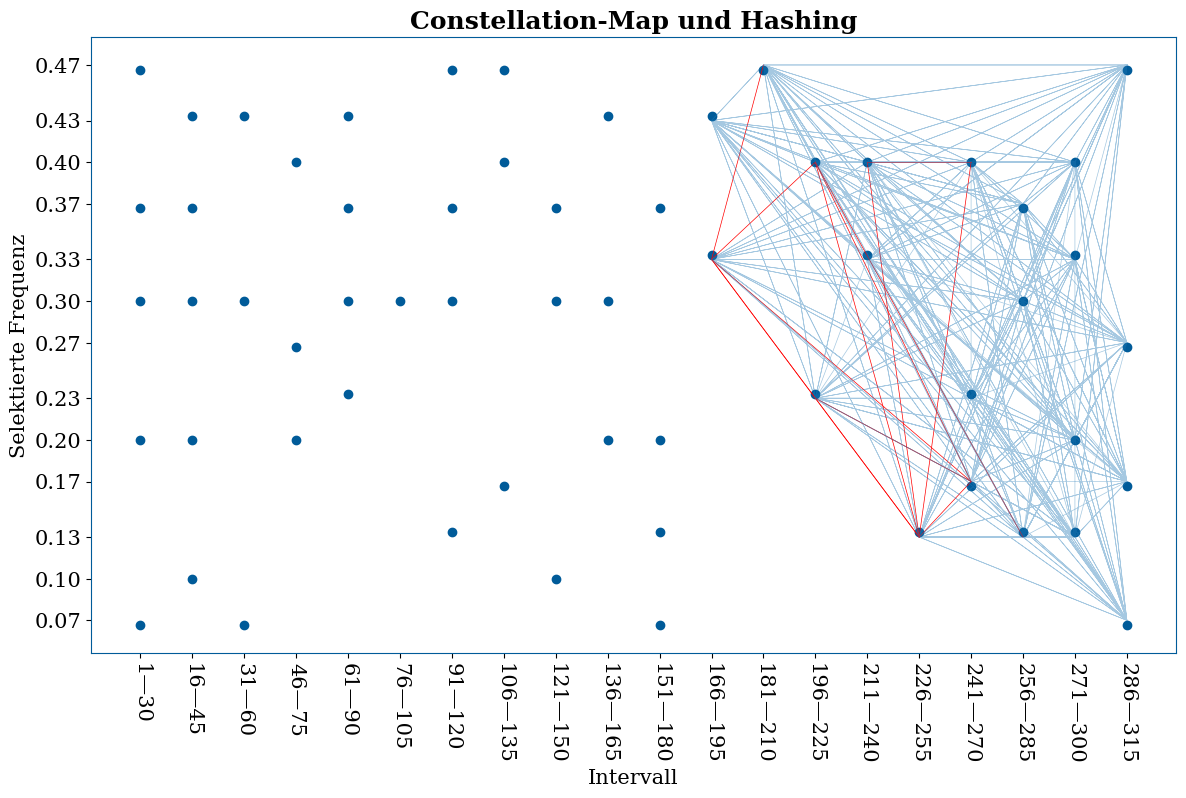
\includegraphics[width=1\textwidth]{plot_method.png}
            \caption{Die Punkte bilden die Constellation-Map. Die zur Übersicht nur rechts eingezeichneten Kanten repräsentieren die Hash-Bildung, wobei rote Kanten ignorierte Hashes darstellen, weil sie mehrfach auftauchen.}
            \label{fig:hashing}
        \end{figure}

        % hierzu ein Plot zur Veranschaulichung der Offsets
        % Scoring/Map-Vergleich
        \vspace{2.25mm}
        \textbf{Single-Protein-Matching:}\ \ Nachdem eine Datenbank mit den Hashes verschiedener Trainings-Proteine (TP) trainiert wurde, wird sie verwendet, um Proteine zu erkennen. Dazu werden für die jeweilige Eingabesequenz von Aminosäuren die Hashes gebildet und deren Positionen gespeichert. Um nun die Ähnlichkeit der Constellation-Map der Eingabe mit denen der TP zu bestimmen, werden pro Eingabe-Hash die Differenzen zwischen dessen Position mit den Positionen der trainierten Hashes gebildet und global pro Protein gezählt. Diese Differenzen repräsentieren den Abstand der Kante in der Eingabe-Map zur Kante der jeweiligen TP-Map, also wie weit die Eingabe-Map verschoben wäre, sollte es sich bei dem TP um das Original handeln. Auf diese Weise sammeln sich pro TP mehrere solcher potentiellen Abstände, wobei nun der Abstand, der am häufigsten aufgetreten ist, offensichtlich die meiste Übereinstimmung in den Kanten zeigt. Diese Tatsache qualifiziert diese Maximalanzahl als geeigneten Score (S1) für ein Match.

        Da es große Proteine mit sehr langen Aminosäuresequenzen kürzere Sequenzen kleinerer funktionsungleicher Proteine enthalten können, reicht der ermittelte Score alleine nicht aus, da in diesem Fall sehr viele Kanten der Eingabe-Map übereinstimmen würden, sodass trotz Mis-Match der nahezu maximale Score erreicht werden würde.

        Um das zu umgehen, wird der Jaccard-Similarity-Index (JSI) verwendet, einem Maß, das die Übereinstimmung zweier Mengen A und B wie folgt bewertet:
        $$JSI(A, B)=\frac{|A \cap B|}{|A \cup B|}$$
        Dieser Index nimmt einen Wert von 0 an, wenn beide Mengen disjunkt sind, und nähert sich der 1 je größer die Schnittmenge ist. Im Fall des Vergleichs zweier Constellation-Maps, also zwei Hash-Mengen, wird hier bewertet, wie viele Kanten sich die beiden Maps positionsunabhängig teilen. Durch diese Unabhängigkeit reicht der JSI alleine nicht als Score aus, sodass nur in Kombination/Multiplikation mit dem S1 ein robuster Score entsteht, da beide zusammen ihre Schwächen aufheben.

        \vspace{2.25mm}
        \textbf{Family-Matching:}\ \ Wenn \protfin\ wie erwartet funktioniert, sollten beim Single-Protein-Matching die Matches mit den besten Scores funktionsähnliche Proteine sein. Ein weiterer Ansatz, solche Verwandten zu ermitteln, ist das Matching mit Proteinfamilien. Hierbei wird als Eingabe eine Tabelle akzeptiert, die lediglich eine Zuordnung von Protein-ID und Familie enthält. Um nun Matches zu finden, werden von allen Hashes einer Familie nur die behalten, die in allen Mitgliedern vorkommen. Anschließend wird die Datenbank nach Proteinen durchsucht, welche ebenfalls diese Hashes enthalten, wobei als Score diesmal nur die Anzahl infrage kommt, wie viele der Hashes enthalten sind. Die Idee hinter dieser Methode ist, dass Proteine derselben Proteinfamilie, also mit ähnlichen Funktionen, möglicherweise familienspezifische Kanten in der Constellation-Map haben.
    % subsection grundalgorithmus (end)
    \subsection{Experiment 1: UniRef90 Sampling} % (fold)
        \label{sub:experiment_1_uniref90_sampling}
        Ein wichtiger Bestandteil des \hyperref[sec:grundalgorithmus]{Algorithmus} ist die Selektion signifikanter Frequenzen zur Erstellung der Constellation-Map. Es wäre möglich, einfach alle Frequenzen auszuwählen und die Signalstärke in den Hash einfließen zu lassen. Problem hierbei ist aber, dass diese Vorgehensweise zu wesentlich mehr Hashes und einer folglich sehr großen Datenbank führt, was wiederum das Scoring/Matching verlangsamt. Ein Anspruch an \protfin\ ist, dass die Datenbankgröße die Eingabegröße nicht wesentlich übersteigt, wobei es sich bei der Eingabe um eine einfache FASTA-Datei handelt.

        Diesem Problem soll durch ein Sampling-Experiment abgeholfen werden. Darin werden aus etwa 180 Millionen Sequenzen je ein zufälliges Intervall für die STFT ausgewählt, transformiert und die Signalstärken je Frequenz gemerkt. Um nun daraus eine Selektionsmethode abzuleiten, werden die Grenzquantile einer jeden Frequenz ermittelt, um signifikant seltene Signalstärken zu ermitteln. Folglich ist es möglich, für die Constellation-Map nur diejenigen Frequenzen zu behalten, welche in den Randzonen der Signalstärken liegen, sodass nicht nur Signale infrage kommen, die für eine besonders starke Ausprägung eines Kidera-Faktors sprechen, sondern auch für den Fall der umgekehrten Ausprägung, wie z.B. Hydrophilie statt Hydrophobie.

        Der Algorithmus wird daher insofern angepasst, dass bei der Frequenz-Selektion von den Maxima der Signalstärken nur die behalten werden, die die Grenzwerte über-/unterschreiten. Zudem wird beim Hashing je Frequenz noch die Information hinzugefügt, ob sie besonders stark oder schwach ist.
    
    % subsection experiment_1_uniref90_sampling (end)
% section material_und_methoden (end)
